\documentclass[12pt]{article}
\usepackage[hmargin=0.75in, vmargin=1in]{geometry}
\geometry{letterpaper}
\usepackage[T1]{fontenc} 
\usepackage[utf8]{inputenc} 
\usepackage[french]{babel}
\usepackage{graphicx} % Support for including images
\usepackage{hyperref} % Support for hyperlinks
\hypersetup{hidelinks = true}
\usepackage{amsmath}
\usepackage{amssymb}
\usepackage{siunitx}
\usepackage{xcolor}
\sisetup{
    round-mode = figures,
    round-precision    = 3           ,
    scientific-notation = true
    }
\usepackage{float}
\usepackage{cancel}
\usepackage{tikz}
\usepackage{booktabs}
\usepackage{comment} 
\usepackage{minted}
\renewcommand{\thesection}{\arabic{section}}
\newcommand*{\rttensor}[1]{\bar{\bar{#1}}}
\newcommand*\circled[1]{\tikz[baseline=(char.base)]{
            \node[shape=circle,draw,inner sep=2pt] (char) {#1};}}
\newcommand\pder[2][]{\ensuremath{\frac{\partial#1}{\partial#2}}} 
\newcommand\pdder[2][]{\ensuremath{\frac{\partial^2 #1}{\partial#2^2}}} 
%------------------------------------------------------------------
% TITLE
%------------------------------------------------------------------
\title{
\centerline{
\includegraphics[width=0.4\textwidth]{images/poly}}
\vspace{0.5 cm}
Projet \\
\vspace{1cm}
ENE6002
\large  \\
Thermohydraulique des systèmes diphasiques \\ 
\Huge-\\
\normalsize Polytechnique Montréal
  }

\author{
    \begin{minipage}{.46\textwidth}
        \begin{center}
            Thomas \textsc{Charpentier} - 2036024\\
            \texttt{thomas.charpentier@polymtl.ca}
        \end{center}
    \end{minipage}%
    \hfill\vrule\hfill
    \begin{minipage}{0.46\textwidth}
        \begin{center}
            Gaétan \textsc{Raynaud} - 2022063\\
            \texttt{gaetan.raynaud@polymtl.ca}
        \end{center}
    \end{minipage}
}    

\date{\today}


%------------------------------------------------------------------
% DOCUMENT START HERE
%------------------------------------------------------------------
\begin{document}
\maketitle
\tableofcontents
\newpage
\section{Introduction et présentation de l'étude\label{section:pres}}

\subsection{Introduction}

Dans les applications industrielles, dès lors que l'on travaille avec un écoulement dans un conduite chauffée, on peut observer en parallèle de la phase liquide l'apparition de vapeur. Entre ces deux phases il s'échange de la masse, de l'énergie et de la quantité de mouvement et le désordre généré s'accompagne généralement d'une chute de pression. Si la conduite est suffisamment longue, la prise en compte des pertes de charges dans un modèle monophasique risque d'être peu représentatif de la réalité, les pertes liées à l'ébullition n'étant pas négligeables.\\

Cette sous-estimation de la perte de pression lors du dimensionnement peut avoir des répercussions sur le rendement de l'installation ou bien sa sécurité. Dans le cas d'un réacteur à eau pressurisé, il est important de connaître les conditions de l'écoulement à tous les endroits de la conduite. On ne souhaite pas se retrouver avec un écoulement diphasique dans une zone où cela n'était pas prévu, avec des conséquences majeures pour la sécurité. De plus les différents scénarios d'accidents (brèche, fusion du coeur...) peuvent placer le système dans des configurations favorables à l'apparition de vapeur qu'il s'agit d'anticiper et de designer convenablement pour s'assurer des marges.\\

Dans le domaine des nouvelles technologies, la micro électronique peut tirer parti d'une bonne utilisation de micro canaux pour dissiper l'énergie lorsque ceci est compliqué (satellites, micro puces...). Ceux-ci possèdent en effet de bien meilleurs coefficients de transfert thermique que les méthodes conventionnelles ce qui permet d'en réduire la taille et potentiellement le coût de fabrication \cite{revellinAdiabaticTwophaseFrictional2007}. Néanmoins la chute de pression doit être évaluée précisément pour assurer un fonctionnement optimal du système de dissipation et cela se traduit par des modèles uni-dimensionnel pour des écoulements diphasiques. \\

%Petroleum engineering cite Shi et al 2005 cf. \href{http://folk.ntnu.no/preisig/HAP_Specials/AdvancedSimulation_files/2014/AdvSim-2014__Matovu_Fahad_Drift-flux\%20models.pdf}{Lien}\\

%Intro de https://doi.org/10.1016/S0017-9310(03)00309-0 

%Citer des applications utiles du calcul de perte de pression dans des écoulements diphasiques, exemples industriels, effet sur le rendement,catastrophes... 
%\textcolor{red}{Parler des codes de calcul courants et des modèles existants}


\subsection{Présentation de l'étude}

Pour ce projet, nous nous intéressons à la perte de pression ainsi qu'au taux de vide moyen pour un écoulement bouillant dans une conduite chauffée. Une représentation d'un banc d'essai typique pour ce type de mesures est disponible à la fig. \ref{fig:instal}

\begin{figure}[ht]%[htbp]
    \centering
    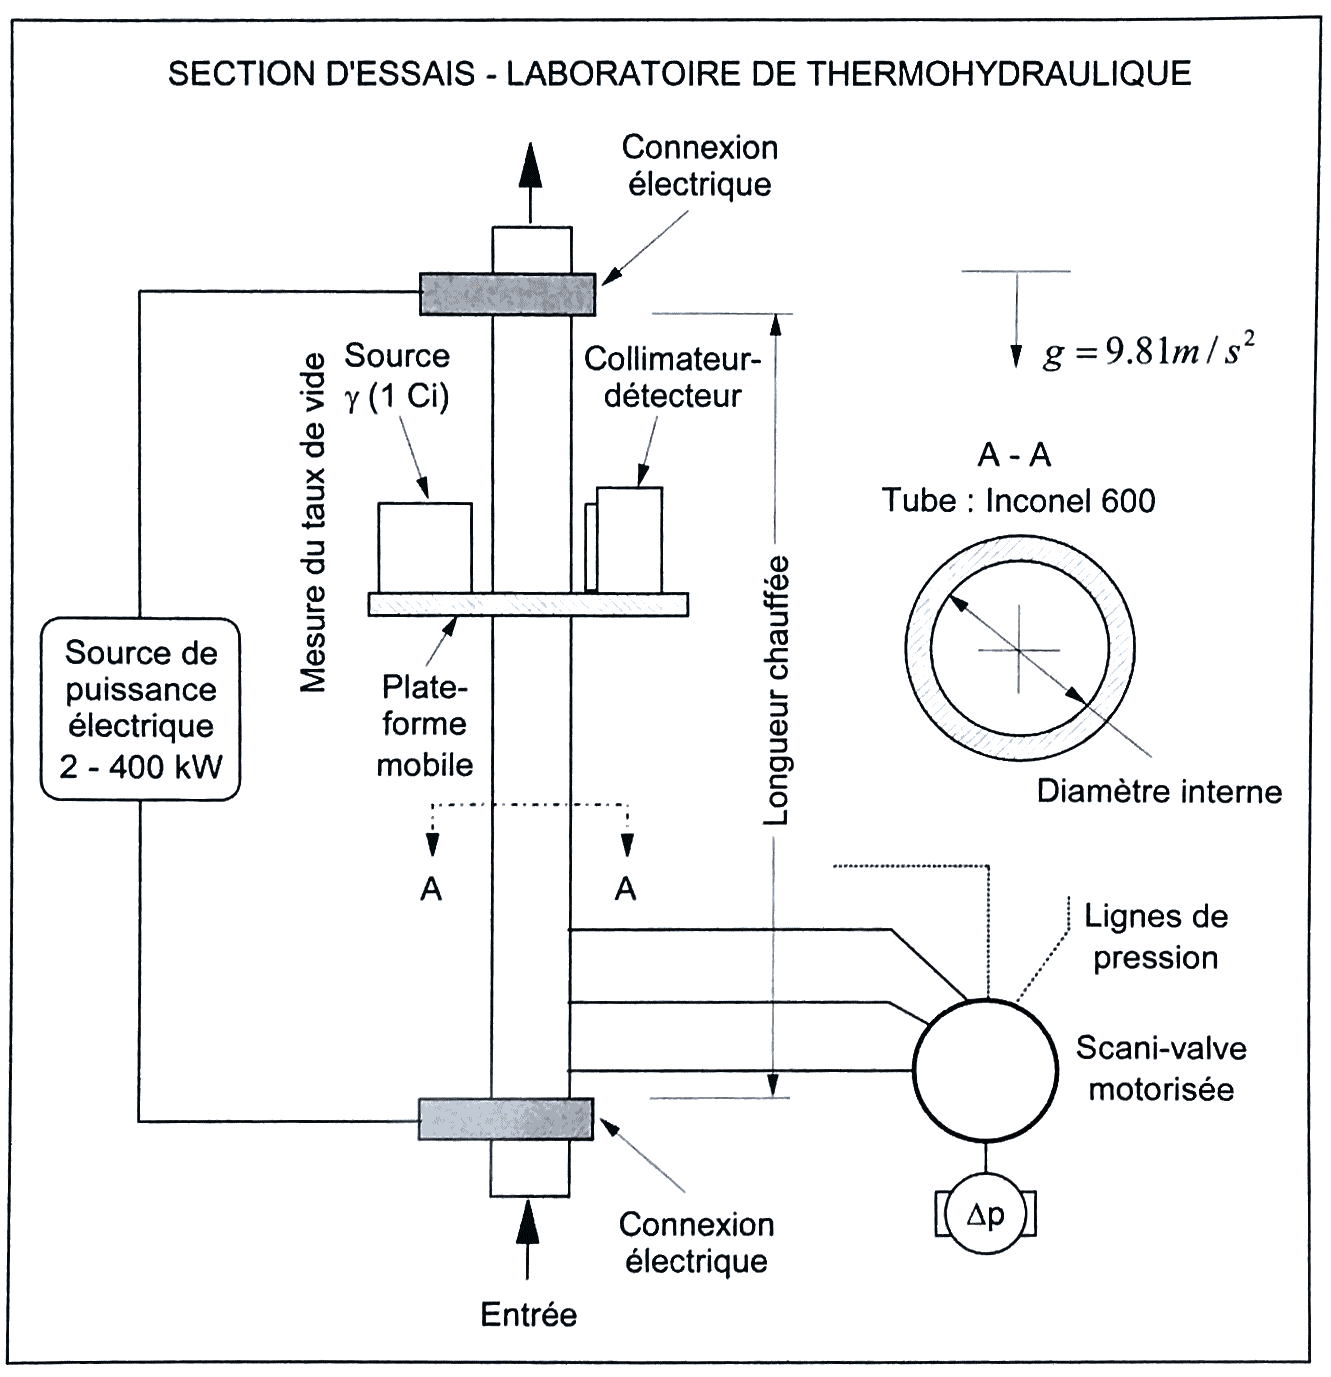
\includegraphics[width=0.7\textwidth]{images/schema_instal.png}
    \caption{Installation pour mesure de perte de pression et du taux de vide - D'après l'énoncé}
    \label{fig:instal}
\end{figure}

Le but de ce projet est de réaliser un modèle numérique et de déterminer les différents paramètres le long de la conduite. L'analyse des résultats se fait en comparant à des tables de données expérimentales. On travaille dans le cas d'un écoulement vertical ascendant.\\ \par
Pour réaliser cela, plusieurs hypothèses ont été réalisées :
\begin{itemize}
    \item \textbf{H1} : L'écoulement est incompressible.
    \item \textbf{H2} : La perte de pression par accélération dans la région non bouillante est négligeable.
    \item \textbf{H3} : La perte de pression totale est négligeable par rapport à la pression de l'écoulement.
    \item \textbf{H4} : L'enthalpie de l'eau sous-refroidie à une température donnée est égale à l'enthalpie de saturation de l'eau correspondant à cette température
\end{itemize}
\vspace{12pt}
\par
La détermination des propriétés thermodynamiques a été faite avec \texttt{pyXSteam}, qui est une librairie Python sur la base de \texttt{X-Steam} disponible sur Excel et Matlab.\\
Le titre et le taux de vide moyen sont déterminés à l'aide des corrélations de \textsc{Chexal-Lellouche} et de \textsc{Inoue}. Le multiplicateur diphasique ainsi que les facteurs de frottements qui servent au calcul de la perte de pression proviennent eux de la corrélation de \textsc{Friedel}.\\ \par






\newpage
\section{Méthode de résolution\label{section:res}}
Afin de trouver la perte de pression dans la conduite, il convient de définir les équations qui régissent le problème.
\subsection{Équations du problème}
Les différentes équations dont on dispose sont :

des équations d'état lors que le mélange est à saturation :
\begin{align}
    T_{sat} &= T_{sat}(P) \\
    h_{l,sat} &= h_{l,sat}(T) = h_{l,sat}(P) \\
    h_{v,sat} &= h_{v,sat}(T) = h_{v,sat}(P)
\end{align}

Des lois de comportement, notamment pour calculer la perte de pression
\begin{equation}
     -\pder[p]{z} = \left(\pder[p]{z} \right)_{a} + \left(\pder[p]{z} \right)_{f} + \left(\pder[p]{z} \right)_{g}
\end{equation}

Que l'on peut écrire comme :
\begin{equation}
    -\pder[p]{z} = \underbrace{\left[\overbrace{\cancel{\frac{\partial}{\partial \tau} G}}^{\text{Ecoul. permanent}}+\frac{\partial}{\partial z} G^{2} v^{\prime}\right]}_{\text{Acceleration}}+\underbrace{\frac{4 \tau_{w}}{D}}_{\text{Frottements}}+\underbrace{\rho_{m} g}_{\text{Gravitation}}
%    -\pder[p]{z} = \phi_{l0}^2 \times \left( \pder[p]{z} \right)_{1\varphi}
\label{eq:pres}
\end{equation}

Avec :
\begin{equation}
    v^{\prime}=\frac{x^{2}}{\varepsilon \rho_{v}}+\frac{(1-x)^{2}}{(1-\varepsilon) \rho_{l}}
\end{equation}

Etant donné la complexité de gérer les cas $\varepsilon \rightarrow 0$ et $\varepsilon \rightarrow 1$ dans l'équation précédente, on a utilisé une équation dérivée du modèle homogène pour $v'$ :

\begin{equation}
    v^{\prime} = \frac{1}{\rho_m} = \frac{1}{\varepsilon \rho_v + (1-\varepsilon)\rho_l }
\end{equation}

Le terme de frottement pouvant être écrit comme la perte de pression (par frottement) si l'écoulement était seulement liquide et une correction, le \og multiplicateur diphasique \fg{}. Ce dernier sera obtenu par la corrélation de \textsc{Friedel} rappelée dans \cite{revellinAdiabaticTwophaseFrictional2007}.
\begin{equation}
    \left(\pder[p]{z} \right)_{f} = f\frac{G^2}{2 \rho_l}\frac{1}{D} \phi_{lo}^2
\end{equation}

où $f$ est défini par :
\begin{equation}
    f = 0.316 \left[\text{Re}_L\right]^{-0.25} = 0.316 \left[\frac{G D}{\mu_l}\right]^{-0.25} 
\end{equation}
On peut donc écrire la perte de pression que nous allons évaluer comme :
\begin{equation}
     -\pder[p]{z} = G^2\pder{z}\left[\frac{1}{\varepsilon \rho_v + (1-\varepsilon)\rho_l } \right] + f\frac{G^2}{2 \rho_l}\frac{1}{D} \phi_{lo}^2 + \left[ \varepsilon \rho_v + (1-\varepsilon)\rho_l  \right] g
\end{equation}


On dispose ensuite d'une relation entre le taux de vide moyen $\varepsilon$ et le titre de l'écoulement $x$ provenant du modèle à vitesses séparées. Il est accompagné de lois de comportements pour fixer les constantes de corrélation :
\begin{equation}
        \frac{1}{\varepsilon} = \frac{\rho_g}{\hat{x} G} <V_{gj}>_{2g} + C_0\left(\frac{\rho_g}{\rho_l}\frac{1-\hat{x}}{\hat{x}} + 1\right) 
\label{eq:DriftFluxModel}
\end{equation}
\begin{align*}
         C_0 \text{ et } <V_{gj}>_{2g} \textnormal{ fonctions des paramètres de l'écoulement selon un modèle} 
\end{align*}

En pratique on l'utilisera de deux manières. Dans l'algorithme classique, on s'en sert pour obtenir $\varepsilon$ à partir de $x$ et $p$ avec l'inverse de l'équation \ref{eq:DriftFluxModel}. Dans le PINN, on utilise plutôt la forme suivante où on retourne $x$ à partir d'un set initial de $\varepsilon,x$ et $p$ :

\begin{equation}
    x = \varepsilon \left[ \frac{\rho_g}{G}<V_{gj}>_{2g} + C_0 \left( \frac{1-x}{\rho_l}\rho_g + x\right) \right]
\end{equation}

Il faut bien noter que $C_0$ et $<V_{gj}>$ dépendent des solutions $\varepsilon,x$ et $p$ ainsi que des propriétés thermodynamiques qui varient elles-même avec les solutions, d'où la complexité du problème. En particulier on a vérifié les versions des corrélations utilisées avec l'Appendix de l'article suivant \cite{coddingtonStudyPerformanceVoid2002}. En effet nous avons relevé quelques erreurs dans la version proposée dans l'énoncé.\\ 

Enfin on utilise des lois de conservation, notamment de la masse qui permet de fixer $G$ pour tout le problème :
\begin{equation}
    \pder[G]{z} = 0
\end{equation}

et de l'énergie du mélange :
\begin{equation}
    \pder{z} \left[ h_{l,sat}(T_{(z)})+x_{(z)}h_{vl,sat}(T_{(z)})\right] = \frac{4}{DG}q''
\label{eq:titre}
\end{equation}

où $q''$ est le flux de chaleur ajouté en paroi obtenu en supposant la puissance thermique $P_{th}$ apportée uniformément répartie sur la longueur chauffée $L_x$ du cylindre : $q'' = \frac{P_{th}}{\pi DL_c}$. On suppose que l'on travaille à saturation, où la pression $p$ et la température $T$ sont directement liées. Ainsi nous n'avons pas besoin de résoudre explicitement $T = T_{sat}(p_{(z)})$\\ \par

\newpage
\section{Zone de saturation\label{section:sat}}
Comme nous négligeons la perte de pression par accélération dans la zone où l'ébullition est sous-refroidie (\textbf{H2}), il nous faut calculer la position où le fluide est à température de saturation. Cela correspond d'ailleurs à l'endroit où le titre thermodynamique devient nul. Pour cela plusieurs méthodes sont possibles.

\subsection{Puissance chauffage}
On peut écrire que la puissance nécessaire pour arriver à la température de saturation en partant de la température d'entrée. Cette puissance dépend du flux massique et de la capacité thermique massique de l'eau. Il s'agit donc de faire un bilan énergétique sur le fluide qui passe dans la conduite. On a :
\begin{equation}
    \dot{Q}_{sat} = \dot{m} Cp \Delta T
\end{equation}
Le terme $Cp$ pouvant être pris pour de l'eau à saturation à la pression de sortie (la variation est faible pour un $\Delta T$ de cet ordre de grandeur), et le terme $\Delta T$ correspond à la différence entre la température de saturation du fluide à la pression donnée et la température d'entrée.\\ 
Comme on considère que la conduite est chauffée uniformément, le rapport entre puissance nécessaire pour arriver à saturation et puissance totale thermique ajoutée $P_{th}$ est égale au rapport entre $L_{sat}$ et longueur totale chauffée $L_c$. On a alors :
\begin{equation}
    L_{sat}= \frac{ \dot{Q}_{sat}\times L_c}{P_{th}}
\end{equation}

\subsection{Différence enthalpie}
Dans les notes de cours, on peut trouver à la page 181, une expression qui nous donne $L_{SC}$, la longueur \emph{subcooled}. Elle s'écrit comme :
\begin{equation}
 L_{s c} = \left(h_{l, s a t} - h_{i}\right)\frac{\dot{m}}{\pi D q_{w}^{\prime \prime}} 
\end{equation}
Cette équation prend mieux en compte les variations des propriétés du fluide avec la température.
\\
Le terme $q_{w}^{\prime \prime}$ correspondant à la puissance de chauffage par unité de surface sur le tube :
\begin{equation}
    q_{w}^{\prime \prime} = \frac{P}{S_{\text{paroi}}} = \frac{P}{\pi D L }
\end{equation}
On peut maintenant s'intéresser aux valeurs prises par les deux termes d'enthalpies.\\ \par
L'enthalpie à saturation $h_{l, s a t}$ est simple à trouver, il s'agit de prendre l'enthalpie à saturation pour la pression de sortie donnée. La perte de pression que l'on cherche à quantifier est trop faible pour pour faire apparaître des variations notables dans la valeur de l'enthalpie à saturation.\\ \par
Pour ce qui est de l'enthalpie d'entrée $h_{i}$, l'hypothèse \textbf{H4} nous indique d'utiliser l'enthalpie à saturation pour cette température.\\
Notons qu'il est possible de travailler avec la \og vraie \fg{} enthalpie en utilisant la température d'entrée et pression corrigée avec la perte de pression expérimentale.
\subsection{Comparaison des méthodes}
Comme nous avons les données pour 2 expériences, nous allons pouvoir comparer les deux méthodes.
Rappelons les différentes valeurs caractéristiques pour ces dernières.
\begin{table}[H]
\caption{Paramètres pour les deux expériences}
\vspace{5pt}
    \centering
    \begin{tabular}{@{}lll@{}}
        \toprule
               & \textbf{Expérience 65BV}& \textbf{Expérience 19}\\
        \midrule
          \textbf{Diamètre} (\si{m}) & \num{13.4e-3} & \num{22.9e-3} \\
          \textbf{Longueur chauffée} (\si{m}) & 1.8 & 1.8 \\
          \textbf{Puissance thermique} (\si{kW}) & 250 & 151,8 \\
          \textbf{Débit massique} (\si{kg/s})& \num{0,64} & \num{0.47} \\
          \textbf{Température entrée} (\si{\celsius})& 184 & 215.3 \\
          \textbf{Pression sortie} (\si{bar})& 20.3 & 42.1 \\
        \bottomrule  
    \end{tabular}
    \label{donnes}
\end{table}

On peut déterminer des valeurs pour $Cp$ de l'eau à saturation basés sur la pression de sortie, ainsi que la température de saturation. On a alors :
\begin{table}[H]
\caption{$Cp$ et $T_{sat}$ pour les deux expériences}
\vspace{5pt}
    \centering
    \begin{tabular}{@{}lll@{}}
        \toprule
               & \textbf{Expérience 65BV}& \textbf{Expérience 19}\\
        \midrule
          \textbf{Cp} (\si{kJ/kg K}) & \num{4.575} & \num{4,901} \\
          \textbf{Température de saturation} (\si{\celsius}) & 212.1 & 253.3 \\
        \bottomrule  
    \end{tabular}
    \label{donnes}
\end{table}

On trouve alors $\dot{Q}_{sat}$ et on en déduit la longueur nécessaire pour atteindre un titre nul.
\begin{table}[H]
\caption{Puissance et longueur sous-refroidie pour les deux expériences}
\vspace{5pt}
    \centering
    \begin{tabular}{@{}lll@{}}
        \toprule
               & \textbf{Expérience 65BV}& \textbf{Expérience 19}\\
        \midrule
          \textbf{Puissance nécessaire} $\dot{Q}_{sat}$ (\si{kW}) & 81.7 & 77.6 \\
          \textbf{Longueur sous-refroidie} $L_{sc}$ (\si{m}) & 0.59 & 0.92 \\
        \bottomrule  
    \end{tabular}
    \label{donnes}
\end{table}

On peut maintenant passer à la seconde méthode avec les enthalpies. On a :
\begin{table}[H]
\caption{Enthalpies pour les deux expériences}
\vspace{5pt}
    \centering
    \begin{tabular}{@{}lll@{}}
        \toprule
               & \textbf{Expérience 65BV}& \textbf{Expérience 19}\\
        \midrule
          \textbf{Enthalpie saturation} $h_{l,sat}$ (\si{kJ/kg}) & 912 & 1102 \\
          \textbf{Enthalpie entrée} $h_{i}$ (\si{kJ/kg}) & 781.2 & 922.6 \\
          \textbf{Enthalpie entrée corrigée} $h_{i,cor}$ (\si{kJ/kg}) & 781.6 & 922.5 \\          
        \bottomrule  
    \end{tabular}
    \label{donnes}
\end{table}

Après application numérique on a alors :
\begin{table}[H]
\caption{Longueurs sous-refroidie pour les deux expériences}
\vspace{5pt}
    \centering
    \begin{tabular}{@{}lll@{}}
        \toprule
               & \textbf{Expérience 65BV}& \textbf{Expérience 19}\\
        \midrule
          \textbf{Longueur sous-refroidie} $L_{sc}$ (\si{m}) & 0.602 & 0.999 \\
          \textbf{Longueur sous-refroidie corrigée} $L_{sc,cor}$ (\si{m}) & 0.600 & 1.000 \\
        \bottomrule  
    \end{tabular}
    \label{donnes}
\end{table}

On remarque que les résultats avec les deux méthodes donnent des valeurs du même ordre de grandeur, ce qui confirme que les deux comparent bien les mêmes choses. De plus les résultats pour les enthalpies, qu'elles soient corrigées ou non sont très proche, l'hypothèse \textbf{H4} est donc cohérente.\\ \par
La différence des résultats entre les deux méthodes est que dans la première, on ne prend pas en compte le changement des propriétés thermiques ($Cp$) du fluide dans la conduite et on travaille seulement avec la valeur à saturation. Il pourrait être plus réaliste de moyenner avec la valeur à l'entrée ou bien de faire l'intégrale sur toute la zone en considérant que le gradient de température est constant dans la conduite.
%\newpage
%\section{Question 4\label{section:ex4}}


\colorlet{droplet color}{blue!50!cyan!80}
\tikzset{%
  raindrop/.pic={
    code={\tikzset{scale=1/10}
 \shade [shading=droplet]
 (0,0)  .. controls ++(0,-1) and ++(0,1) .. (1,-2)
 arc (360:180:1)
 .. controls ++(0,1) and ++(0,-1) .. (0,0) -- cycle;
  }}}

\begin{figure}[H]
\begin{center}
\begin{tikzpicture}[line join=round,rotate=270]
\filldraw[draw=black,ultra thick,fill=droplet color!20]
 (0,12) arc[x radius=2, y radius=0.4, start angle=180, end angle=0]
 (4,12) arc[x radius=2, y radius=0.4, start angle=0, end angle=-180];
\filldraw[ultra thick,fill=droplet color!70,opacity=1,fill opacity=0.7]
  (0,12) -- 
  (0,0) 
  arc[x radius=2, y radius=0.4, start angle=-180, end angle=0] --
   (4,12)
  arc[x radius=2, y radius=0.4, start angle=0, end angle=-180];
\draw[dashed] 
  (0,0) arc[x radius=2, y radius=0.4, start angle=180, end angle=0];

%\draw[red,<->, thick] (0,9) -- (1,9)node[right] {$R$}-- (2,9);
\draw[black,->,dotted] (-1.5,1.5) -- (-0.05,1);
\draw[black,->,dotted] (-1.5,3.5) -- (-0.05,3);
\draw[black,->,dotted] (-1.5,5.5) -- (-0.05,5);
\draw[black,->,dotted] (-1.5,7.5) -- (-0.05,7);
\draw[black,->,dotted] (-1.5,9.5) -- (-0.05,9);
\draw[black,->,dotted] (-1.5,11.5)node[above left]{$P = 150 \si{kW}$} -- (-0.05,11);

\draw[black,->,dotted] (5.5,1.5) -- (4.05,1);
\draw[black,->,dotted] (5.5,3.5) -- (4.05,3);
\draw[black,->,dotted] (5.5,5.5) -- (4.05,5);
\draw[black,->,dotted] (5.5,7.5) -- (4.05,7);
\draw[black,->,dotted] (5.5,9.5) -- (4.05,9);
\draw[black,->,dotted] (5.5,11.5) -- (4.05,11);

\draw[black,->,thick] (1,-1.5) -- (1,-0.5);
\draw[black,->,thick] (2,-1.5)node[left]{Inlet} -- (2,-0.5);
\draw[black,->,thick] (3,-1.5) -- (3,-0.5);

\draw [thick,red] [<->] (0,13) --++(2,0) node [right] {$\varnothing = 13,3 \si{mm}$} --++(2,0);
\draw [thick] [<->] (6,0) --++(0,6) node [below] {$L=1,90 \si{m} $}--++(0,6);
%\draw [thick] [->] (1,10.5) --++(-0.5,-0.4) node [below left]
%{$\vec{e_{\theta}}$};
%\draw[dashed] (2,9.9)--(1.5,10.2)node [right]{$r$}-- (1,10.5);


%\draw[black,dotted, thick] (0,2) -- (4,2);
%\draw[black,dotted, thick] (0, 2) .. controls(1,4) and (3,4) .. (4, 2);
%\draw[black,->, thick] (1,2) -- (1,3.1);
%\draw[black,->, thick] (3,2) -- (3,3.1);
%\draw[black,->, thick] (2,2) -- (2,3)node[below] {$\vec{u}$} -- (2,3.5);
%\draw[black,->, thick]    (2.5,3) -- (2.5,4)node[below] {$\dot{Q}_G = 0,002$ \si{m^3/s}} -- (2.5,5);
\end{tikzpicture}

\caption{Schéma de la conduite pour étudier la chute de pression}
    \label{fig:ConfigExo4}
    \end{center}
\end{figure}

Dans cet exercice, nous travaillons avec une conduite chauffée uniformément par une puissance $P = 150 \si{kW}$ comme représentée sur la fig. \ref{fig:ConfigExo4}. Les paramètres à l'entrée de la conduite (noté Inlet sur le schéma) sont donnés comme :

\begin{equation}
    \left\{
    \begin{array}{r c l l}
    P &=& 30 & \si{bar} \\
    T_{SR} &=& 10 & \si{K}\\
    \dot{m} &=& 0.42 &\si{kg/s}
    \end{array}
    \right.
\end{equation}
\\
On rappelle les hypothèses utilisés dans ce problème :
\begin{itemize}
    \item \textbf{H1} : L'écoulement est incompressible.
    \item \textbf{H2} : La perte de pression par accélération dans la région non bouillante est négligeable.
     \item \textbf{H3} : La perte de pression totale est négligeable par rapport à la pression de l'écoulement.
\end{itemize}
\vspace{12pt}
\par
\subsection{Titre thernodynamique nul - $x$}
Comme il y a une température de sous-refroidissement $T_{SR}$ en entrée, la température de saturation de l'eau à 30 \si{bar} (qui est égale à 233,7\degre C) n'est atteinte que plus loin dans la conduite. On cherche donc la distance qu'il faut pour réchauffer l'écoulement de 10 \si{K}, qui correspond à l'endroit où le titre thermodynamique est nul.
On peut écrire :
\begin{equation}
    \dot{Q}_{sat} = \dot{m} Cp \Delta T
\end{equation}
Le terme $Cp$ pouvant être pris pour une pression de 30 \si{bar}, il vaut alors 4715,9 \si{kJ/kg K}. On a trouve alors que la puissance nécessaire est de :
\begin{equation}
    P_{sat} = 19.8 \si{kW}
\end{equation}
Comme on considère que la conduite est chauffée uniformément, le rapport entre puissance nécessaire pour arriver à saturation et puissance totale thermique ajoutée $P_{th}$ est égale au rapport entre $L_{sat}$ et longueur totale chauffée $L_c$. on a alors :
\begin{equation}
\boxed{
    L_{sat}= \frac{ P_{sat}\times L_c}{P_{th}} = \frac{19.8 \times 1,9}{150} = 0.25~\si{m} 
    }
\end{equation}
\subsection{Titre thermodynamique en sortie - $x_s$}
Nous pouvons donc maintenant nous concentrer sur l'obtention du titre en sortie de la conduite.\\
La conservation de l'énergie nous donne la forme suivante pour le titre :
\begin{equation}
    x_s = \frac{4}{G}\frac{1}{D}\frac{q''}{h_{lv,sat}}L
\end{equation}
Cette forme est valable à partir du moment où le titre est nul. Dans notre cas, la conduite ne fait donc plus L = 1.9 \si{m} mais il faut lui enlever la région non-bouillante qui fait 0.25 \si{m}.\\ \par
Définissons maintenant les termes que nous avons besoin pour cette équation. Commençons par les surfaces, il y a la surface de la paroi et la section de la conduite qui donnent respectivement :
\begin{equation}
    S_{par} = L_c \times \pi D = \num{0.0794}~\si{m^2}
\end{equation}

\begin{equation}
    S_{con} = \frac{\pi D^2}{4} = \num{1.3894e-4}~\si{m^2}
\end{equation}
On peut ainsi définir le flux massique $G$ :
\begin{equation}
    G = \frac{\dot{m}}{S_{con}} = \num{3023.13} ~\si{kg/m^2s}
\end{equation}
Et $q''$ le flux de chaleur sur la paroi :
\begin{equation}
    q'' = \frac{P}{S_{par}} = \num{1889,5} ~\si{kW/m^2}
\end{equation}

Enfin le dernier terme nécessaire est $h_{lv,sat}$ qui est la différence entre l'enthalpie à saturation du gaz et du liquide :
\begin{equation}
    h_{lv,sat} = h_{v,sat} - h_{l,sat} = 2803 -1007,7 = 1795,3 ~\si{kJ/kg}
\end{equation}
Les valeurs proviennent des tables de saturation de l'eau à une pression de 30 \si{bar}.\\
On a alors : 
\begin{equation}\boxed{
    x_s = \frac{4}{G}\frac{1}{D}\frac{q''}{h_{lv,sat}} \left(L_c - L_{sat}\right) = 0,173
    }
\end{equation}
\subsection{Perte de pression totale - $\Delta P$}

On peut désormais s'intéresser à la perte de pression dans la conduite qui est de la forme : 
\begin{equation}
\begin{array}{c}
-\Delta P=\frac{1}{2} f \frac{G^{2}}{\rho_{l}} \frac{L}{D} \overbrace{\left[\frac{1}{x_{e}} \int_{0}^{x_{e}} \phi_{l_{0}}^{2} d x\right]}^{\text{Multiplicateur diphasique}}+\frac{G^{2}}{\rho_{l}}\overbrace{\left[\frac{x_{e}^{2}}{\varepsilon_{e}} \frac{\rho_{l}}{\rho_{v}}+\frac{\left(1-x_{e}\right)^{2}}{\left(1-\varepsilon_{e}\right)}-1\right]}^{\Delta P\text{ par accélération}} \\
+\underbrace{\cancel{\frac{L}{x_{e}} g \int_{0}^{x_{e}}\left[\rho_{v} \varepsilon+\rho_{l}(1-\varepsilon)\right] d x}}_{\text{Conduite horizontale $g=0$}}
\end{array}
\end{equation}

Les termes du \og Multiplicateur diphasique \fg{} et \og Perte de pression par accélération \fg{} sont obtenus par lecture dans des abaques. On peut alors, avec le titre en sortie $x_s=17,3\%$ et $P = 30 ~ \si{bar}$ , en déduire :
\begin{equation}
    \left\{
    \begin{array}{r c l}
    \left[\frac{1}{x_{e}} \int_{0}^{x_{e}} \phi_{l_{0}}^{2} d x\right] &=& 8 \\[2ex]
    \left[\frac{x_{e}^{2}}{\varepsilon_{e}} \frac{\rho_{l}}{\rho_{v}}+\frac{\left(1-x_{e}\right)^{2}}{\left(1-\varepsilon_{e}\right)}-1\right] &=& 4 \\
    \end{array}
    \right.    
\end{equation}
Le terme  noté $f$, correspond au facteur de frottement monophasique, défini comme :
\begin{equation}
    f=0.316\left[\text{Re}_L \right]^{-0.25} = 0.316\left[\frac{(1-x) G D}{\mu_l} \right]^{-0.25}
\end{equation}
%La vitesse moyenne de la phase liquide de l'écoulement se détermine avec le %débit massique :
%\begin{equation}
%    u_l = \frac{\dot{m}}{\rho_l}\frac{1}{S_{con}} = 3.67~ \si{m/s}
%\end{equation}
Et en utilisant les valeurs :
\begin{equation}
    \left\{
    \begin{array}{r c l l}
%    \rho_l &=& 823.1 &\si{kg/m^3}\\
    x &=& 0.173 & \\
    \mu_l &=& \num{116,4e-6} &\si{Pa.s}
    \end{array}
    \right.    
\end{equation}
Nous obtenons, $\text{Re}_L = \num{287493,7}$ soit $f = \num{0,0136}$\\

En injectant le tout dans l'équation de la perte de pression on obtient :
\begin{equation}
    \boxed{
    -\Delta P = \num{130709} ~\si{Pa} = 1.31 ~\si{bar}
    }
\end{equation}
%\newpage
%\section*{Annexes\label{section:annexes}}


\subsection*{Code utilisé pour le problème 3}

{
\scriptsize
\inputminted[
frame=lines,
framesep=2mm,
baselinestretch=1,
linenos
]{python}{Pb3.py}

}

% References
%\bibliographystyle{plain}
%\bibliography{references}
\end{document}
